\documentclass[9pt]{beamer}
% \usetheme{metropolis}
% \usetheme[progressbar=frametitle]{metropolis}
\usetheme[
    progressbar=frametitle,
    block=fill]{metropolis}

\usepackage{appendixnumberbeamer}
\usepackage[round]{natbib}
\usepackage{amssymb, amsthm, mathtools}
\usepackage{amsmath}
\usepackage{color}
\usepackage{colortbl}
\usepackage{algorithm}
\usepackage{algorithmic}
\usepackage{ulem}
\usepackage{accents}
\usepackage{subcaption}
\usepackage{verbatim}
\usepackage{bibentry}
\usepackage{fixltx2e}
\usepackage{relsize}
\usepackage{fancybox}
\usepackage{booktabs}
\usepackage[scale=2]{ccicons}
\usepackage{xspace}
\usepackage{pgfplots}
\usepackage{array, multirow}
\usepackage{numprint}
\usepackage{graphicx}
\usepackage{caption} 
\usepackage{wrapfig}
\usepackage{physics}
\pgfplotsset{compat=1.14}
\usepackage{tikz}
	\usetikzlibrary{positioning}
	\usetikzlibrary{arrows.meta}
\usepgfplotslibrary{dateplot}
\renewcommand{\bibsection}{}
\setbeamertemplate{frametitle continuation}{}

% \setbeamercolor{block body}{bg=mDarkTeal!30}
% \setbeamercolor{block title}{bg=mDarkTeal,fg=black!2}

% \setbeamercolor{block body}{bg=light}
% \setbeamercolor{block title}{bg=light}

\setbeamertemplate{theorems}[numbered]

\newcommand{\yt}{\textit{YouTube-8M}\xspace}

\usetikzlibrary{positioning}
\setbeamercolor{background canvas}{bg=white}

\newtheorem{proposition}{Proposition}[section]

\setbeamertemplate{section in toc}[sections numbered]
\setbeamertemplate{subsection in toc}[subsections numbered]


\title{Understanding and Training Deep Diagonal Circulant Neural Networks}
\author{\textbf{Alexandre Araujo}\inst{1,2}, Benjamin Negrevergne\inst{1},
  Yann Chevaleyre\inst{1} and Jamal Atif\inst{1}}
\date{}
\institute{\inst{1}Université Paris-Dauphine, PSL Research University, CNRS, LAMSADE \\
[1em]\inst{2}Wavestone, Paris, France}

\titlegraphic{
\vspace{21em}
\begin{columns}
  \begin{column}{.18\textwidth}
  
\includegraphics[trim={0 5cm 0 5cm}, width=2cm]{logos/PSL.png}
  \end{column}
  \begin{column}{.18\textwidth}
  
\includegraphics[width=2cm]{logos/dauphine.png}
  \end{column}
  \begin{column}{.18\textwidth}
  
\includegraphics[width=2cm]{logos/lamsade.jpg}
  \end{column}
  \begin{column}{.14\textwidth}
  
\includegraphics[width=1cm]{logos/cnrs.png}
  \end{column}
  \begin{column}{.22\textwidth}
  
\includegraphics[trim={10cm 0 10cm 0}, width=2cm]{logos/wavestone.png}
  \end{column}
\end{columns}
}

\begin{document}

\begin{frame}
    \titlepage
\end{frame}

% \begin{frame}{Overview}
%     \tableofcontents
% \end{frame}


% \section{Introduction to Supervised Learning \& Neural Networks}

\section{Introduction to Neural Networks}

% \begin{frame}{Supervised Learning Algorithms}

% \begin{figure}
%   \begin{minipage}[!ht]{0.42\textwidth}
%   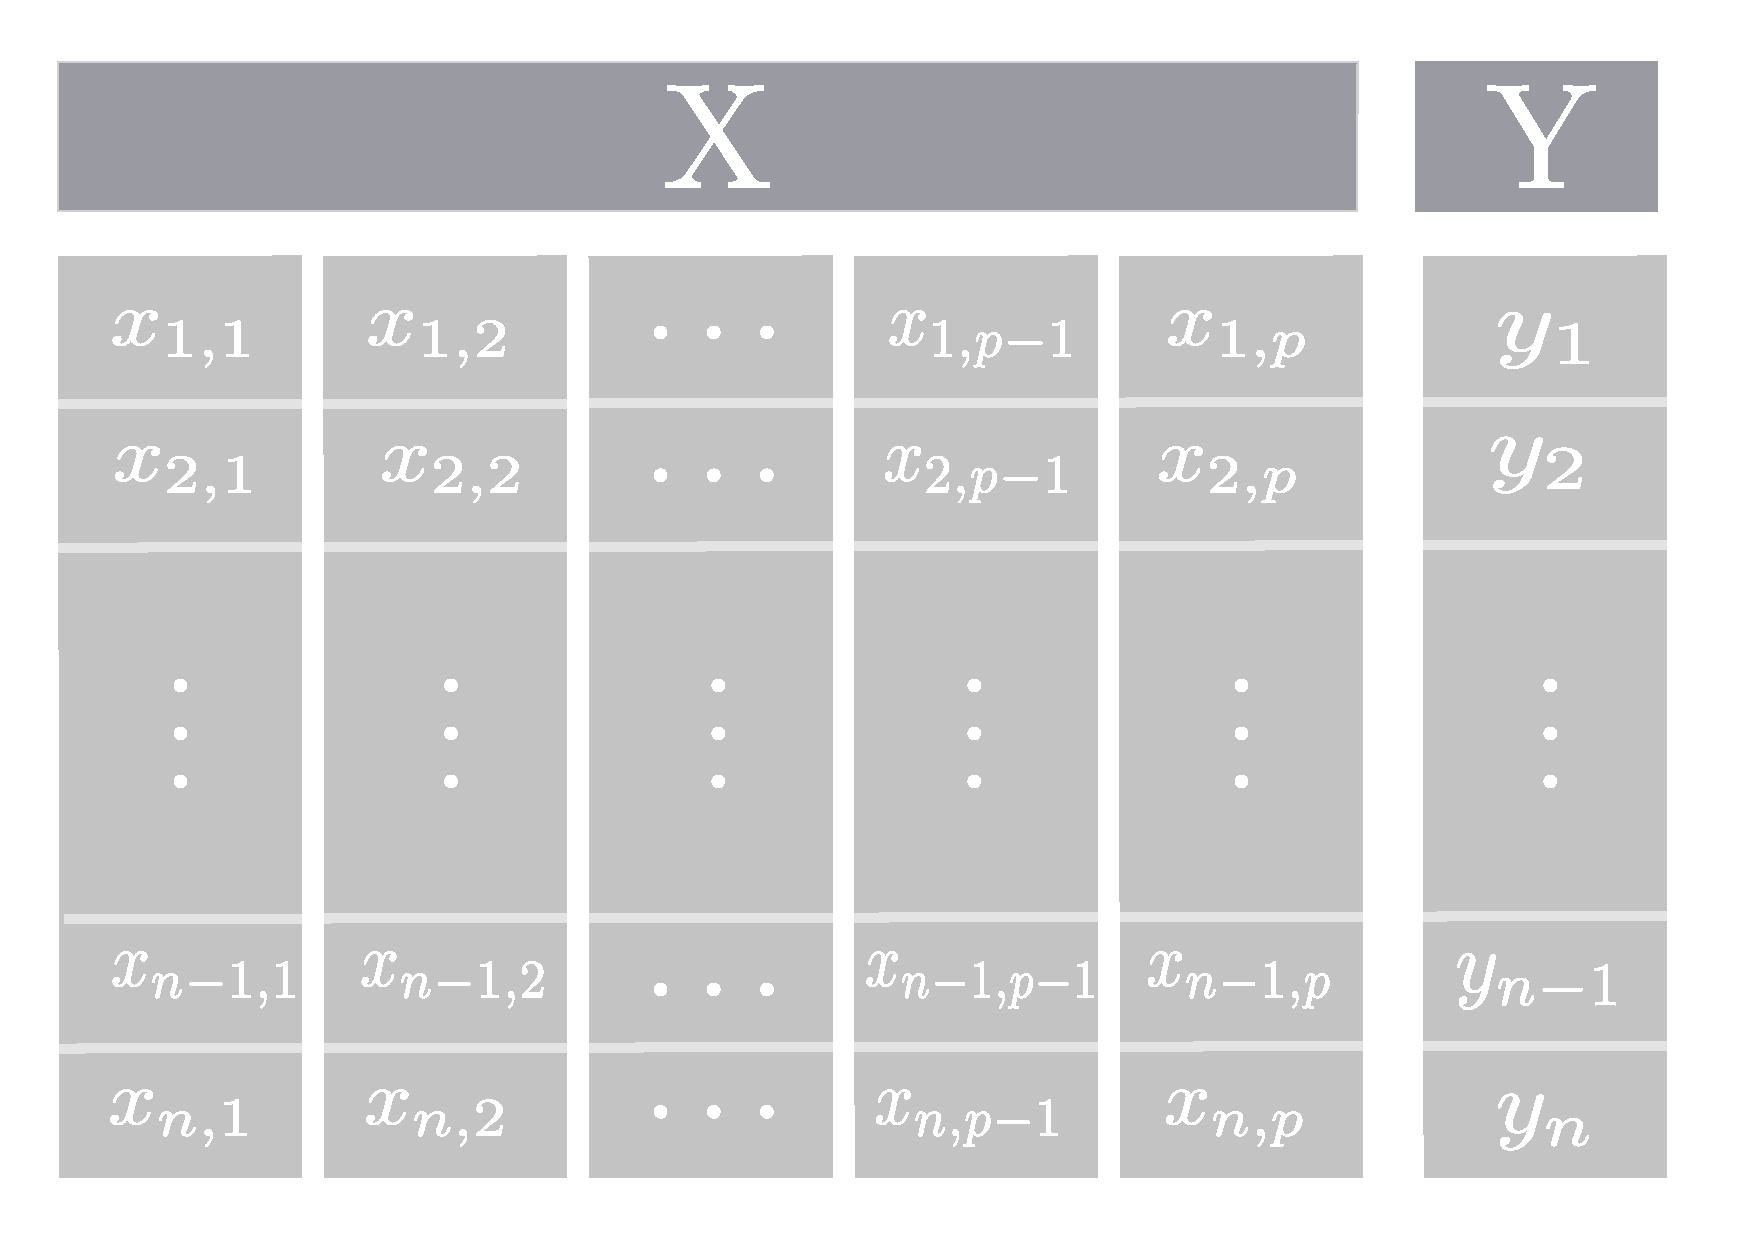
\includegraphics[width=\textwidth]{images/TableauDonneeApprentissage.pdf}
%   \end{minipage} \hspace{0.3cm}
%   \begin{minipage}[!ht]{0.52\textwidth}
%   Given a set of $n$ \textbf{training examples} $\left\{(\mathbf{x}_1, y_1),\dots,(\mathbf{x}_n,y_n)\right\}$ where $\mathbf{x}_i$ is the feature vector of the $i^{th}$ example, and $y_i$ is the corresponding label. \\
%   \textbf{Assumption:} there is a function $f$ matching any feature vector to its label.
%  \end{minipage}
% \end{figure}
%   The goal of a  \textbf{learning algorithm} is to approximate $f$ by a parameterized function $f_{\theta}$.
%   In order to measure how well the function fits, \textbf{a loss function} $\mathcal{L}: \mathcal{Y}\times \mathcal{Y} \rightarrow \mathbb{R}^{+}$ is defined.
%   The standard method to learn the parameter $\theta$ is the \textbf{empirical risk minimization (ERM)}:
% \begin{equation*}
%     \hat{\theta}_{ERM} := \text{argmin}_{\theta}\left[\frac{1}{n} \sum_{ i =1}^{n} \mathcal{L} \left(y_i,f_{\theta}\left(x_i\right)\right)\right]
% \end{equation*}
% \end{frame}
 
 
% \begin{frame}{Deep neural networks}
%          \textbf{Deep neural networks} (large and complex networks) have recently proven outstanding results especially in \textbf{image classification}.
%   \begin{center}
%       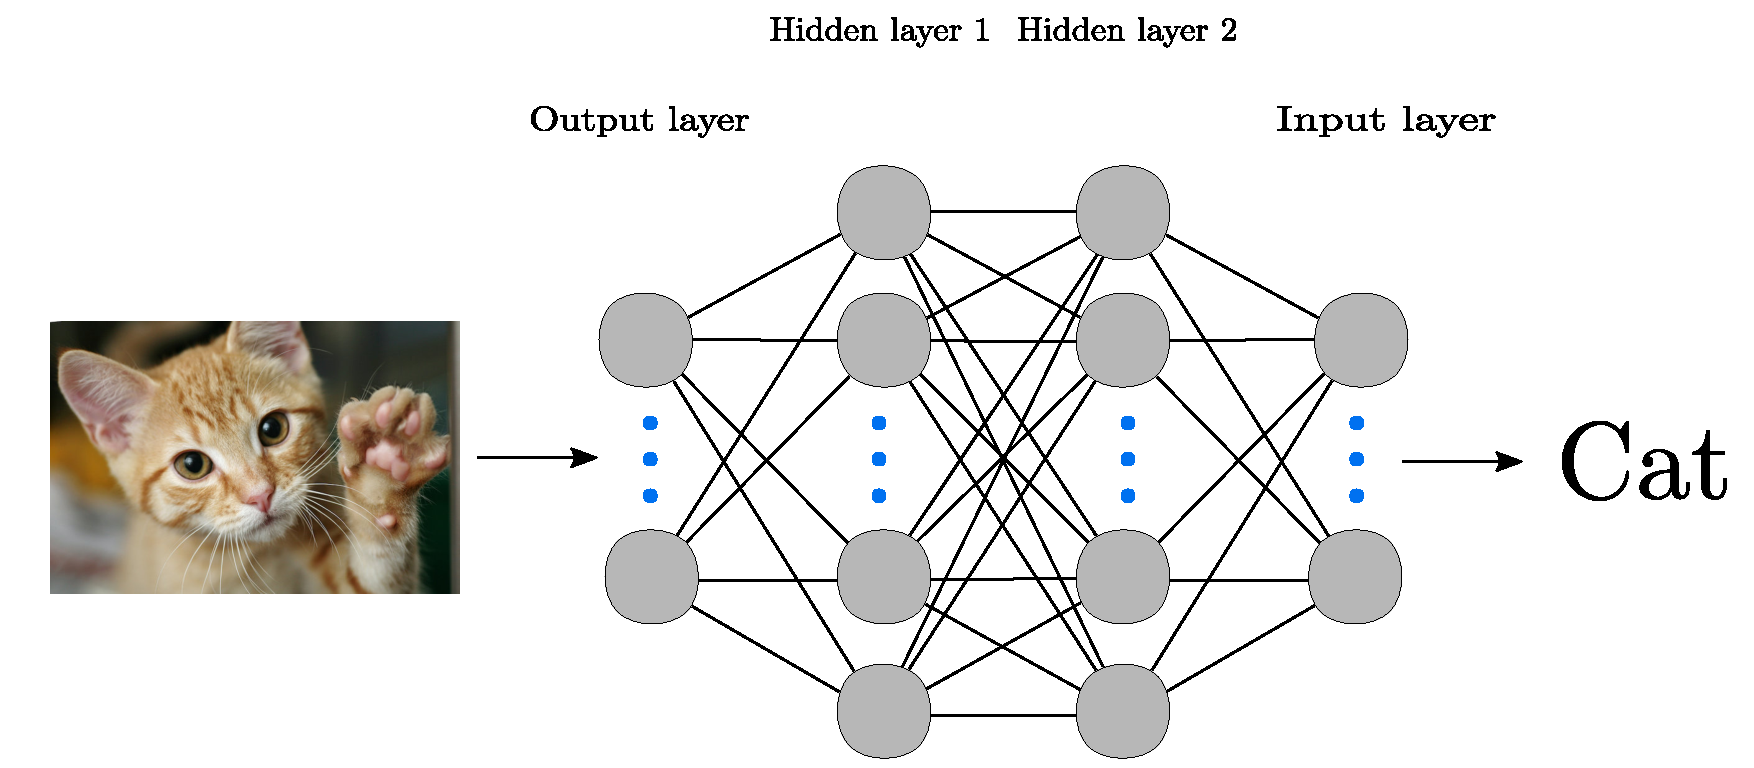
\includegraphics[width=0.8\textwidth]{images/NeuralNet2hiddenLayers.pdf}
%   \end{center}
%   \vspace{-0.5cm}
%      \textbf{No free lunch:} 
%      \begin{itemize}
%          \item[1)] Neural networks (especially deep neural networks) lack theoretical guarantees regarding specification and consistency of the model. 
%          \item[2)] The model is often over-parameterized, which can lead to over-fitting, or to \textbf{major flaws in the classification task} (e.g adversarial examples). 
%      \end{itemize}
% \end{frame}


\begin{frame}{Deep neural networks}

% A \textbf{neural network} is a directed and weighted graph, modeling the structure of a \textbf{dynamic system}. 
A neural network is analytically described by a list of function compositions.

\begin{block}{Fully-connected neural network}
    A fully-connected neural network of $\ell$ layers is defined as follows:
    \begin{equation*}
        \mathcal{N}(x) = \phi^{(\ell)}_{\mathbf{W}_\ell,\mathbf{b}_\ell} \circ \phi^{(\ell-1)}_{\mathbf{W}_{\ell-1},\mathbf{b}_{\ell-1}} \circ \cdots \circ \phi^{(1)}_{\mathbf{W}_1,\mathbf{b}_1}(x)
    \end{equation*}
     where for any $i$, $\phi^{(i)}_{\mathbf{W}_i,\mathbf{b}_i} := z \mapsto \sigma(\mathbf{W}_i \mathbf{z} + \mathbf{b}_i)$, $\mathbf{z}_i \in \mathbb{R}^m$, $\mathbf{b}_i \in \mathbb{R}^m$, $\mathbf{W}_i \in \mathbb{R}^{m \times n}$, and $\sigma$ some non linear (activation) functions.
\end{block}
\textbf{Feed forward networks}, as well as some other specific types of networks are said to be \textbf{universal approximators}~\cite{cybenko1989approximation}.
\end{frame}



\begin{frame}{Context \& Objectives}

\begin{block}{Deep Neural Network are hard to train}
\begin{itemize}
    \item They can have millions (e.g. ResNet \cite{he2016deep}) and sometimes billions of parameters (e.g. GPT-3 \cite{brown2020language})
    \item We don’t know if millions of parameters are necessary 
    \item They are hard to deploy into real world applications
\end{itemize}
\end{block}

\vspace{0.5cm}

\begin{block}{Objective: Reducing the size of a neural network. 2 techniques exist}
\begin{itemize}
    \item  A posteriori compression of neural network models 
    \item Devise compact neural network architecture 
\end{itemize}
\end{block}

$\rightarrow$ We focus on devising compact neural network architecture. 
    
\end{frame}

\section{Building Compact Deep Neural Networks}

\begin{frame}{Model compression for Deep Learning}

\textbf{Constraining the weight representation}
\begin{itemize}
  \item Floating variable with limited precision \cite{Gupta:2015:DLL:3045118.3045303}
  \item Quantization \cite{courbariaux2015binaryconnect,MellempudiKM0KD17, rastegariECCV16}
  \item Hashing techniques \cite{chen2015hashing}
\end{itemize}
 
\textbf{Matrix factorization}
\begin{itemize}
  \item Use of low rank matrices and decomposition as weights matrices \cite{NIPS2013_5025, Jaderberg2014SpeedingUC, 8099498}
\end{itemize}

\textbf{Imposing structures on weight matrices}
\begin{itemize}
    \item Use structured matrices instead of Dense Matrices \cite{7410684,NIPS2015_5869}
\end{itemize}

\end{frame}


\begin{frame}{Circulant matrices for Deep Learning}
A n-by-n circulant matrix $\mathbf{C}$ is a matrix  where each row is a cyclic right shift of the previous one as illustrated below.
\begin{equation*}
    \mathbf{C} = \text{circ}(\mathbf{c}) = \begin{pmatrix} \vspace{0.1cm}
    c_0 & c_{n-1} & c_{n-2} & \dots & c_1 \\ \vspace{0.1cm}
    c_1 & c_0 & c_{n-1}  & & c_2 \\ \vspace{0.1cm}
    c_2 & c_{1} & c_{0} & & c_3 \\ \vspace{0.1cm}
    \vdots & & & \ddots  & \vdots \\ \vspace{0.1cm}
    c_{n-1} & c_{n-2} & c_{n-3} & & c_0
    \end{pmatrix}
\end{equation*}
\begin{block}{Advantages:}
  \begin{itemize}
  \item The circulant matrix $\mathbf{C} \in \mathbb{R}^{n\times n}$ can be \textbf{compactly represented in memory} using only $n$ real values instead of $n^2$.
  \item Multiplying a circulant matrix $\mathbf{C}$ by a vector $\mathbf{x}$ \textbf{can be done efficiently in the Fourier domain}
  \end{itemize}
\end{block}

% \begin{block}{Disavantages:}
%   \begin{itemize}
%   \item The circulant matrix $C \in \mathbb R^{n\times n}$ can be \textbf{compactly represented in memory} using only $n$ real values instead of $n^2$.
%   \item Multiplying a circulant matrix $C$ by a vector $x$ \textbf{can be done efficiently in the Fourier domain}
%   \end{itemize}
% \end{block}


\end{frame}



\begin{frame}{Efficiency of operation with Circulant Matrices}
    
    A circulant matrix $\mathbf{C} \in \mathbb{R}^{n \times n}$ such as $\mathbf{C} = \text{circ}(\mathbf{c})$ can be diagonalized by the Discrete Fourier Transform:
    \begin{equation*}
        \mathbf{C} = \mathbf{W}^{-1} \Lambda \mathbf{W}
    \end{equation*}
    where $\mathbf{W} = \frac{1}{\sqrt{n}} \left( \omega^{jk} \right)_{j,k = 0, \dots, n-1}$ with $\omega$ being the $n^{th}$ root of unity and $\Lambda$ is a diagonal matrix with the eigenvalues of the matrix $\mathbf{C}$. \\ \vspace{0.8cm}
    
    Therefore, the operation can be done efficiently with the \textbf{Fast Fourier Transform} as follows:
    \begin{equation*}
        \mathbf{C}\mathbf{x} = \text{IDFT}( \text{DFT}(\mathbf{c}) * \text{DFT}(\mathbf{x}) )
    \end{equation*}
    where the multiplication is performed elements-wise. 
\end{frame}


% \begin{frame}{Circulant matrices for Deep Learning}

% The fully connected layers are then represented as follows:
% \begin{equation*}
% 	h(x) = \phi\left(\left[\prod_{i=1}^{k} D^{(i)} C^{(i)}\right]x + b\right)
% \end{equation*}
% \noindent
% where the parameters of each matrix $D^{(i)}$ and $C^{(i)}$ are trained using a gradient based optimization algorithm, and $k$ defines the number of factors we choose for the training. 
% \end{frame}



\begin{frame}{Relation between diagonal circulant matrices and low rank matrices}

\begin{theorem}[Reformulation from \citet{Huhtanen2015}] 
For every matrix $\mathbf{A} \in \mathbb{C}^{n \times n}$, for any $\epsilon > 0$, there exists a sequence of matrices $\mathbf{B}_1 \cdots \mathbf{B}_{2n-1}$ where $\mathbf{B}_i$ is a circulant matrix if $i$ is odd, and a diagonal matrix otherwise, such that $\norm{\mathbf{B}_1 \mathbf{B}_2 \cdots \mathbf{B}_{2n-1} - \mathbf{A}} < \epsilon$.
\end{theorem}

\vspace{0.5cm}

This theorem is of little use to understand the expressive power of diagonal-circulant matrices when they are used in deep neural networks:
\begin{itemize}
    \item The bound only depends on the dimension of the matrix $\mathbf{A}$
    \item The theorem does not provide any insights regarding the expressive power of $m$ diagonal-circulant factors when $m$ is much lower than $2n - 1$
\end{itemize}
\end{frame}

\begin{frame}{Relation between diagonal circulant matrices and low rank matrices}
    
\begin{theorem}[Rank-based circulant decomposition] Let $\mathbf{A} \in \mathbb{C}^{n \times n}$ be
a matrix of rank at most $k$. Assume that $n$ can be divided by $k$. For
any $\epsilon > 0$, there exists a sequence of $4k+1$ matrices $\mathbf{B}_{1}, \dots, \mathbf{B}_{4k+1},$ where $\mathbf{B}_{i}$ is a circulant matrix if $i$ is odd, and a diagonal matrix otherwise, such that $\norm{\mathbf{B}_1\mathbf{B}_2 \dots \mathbf{B}_{4k+1} - \mathbf{A}} < \epsilon$
\end{theorem}

\vspace{0.5cm}

A direct consequence of this theorem, is that if the number of diagonal-circulant factors is set to a value $K$, we can represent all linear transform whose rank is $\frac{K - 1}{4}$.
\end{frame}

\begin{frame}{Diagonal-Circulant Neural Network}

We replace the weight matrices of Fully-Connected layers by a product of Diagonal and Circulant matrices :

\begin{block}{Fully-Connected layer}
\begin{equation*}
    \phi_{\mathbf{W},\mathbf{b}} := z \mapsto \sigma(\mathbf{W} \mathbf{z} + \mathbf{b})
\end{equation*}
where $\mathbf{z} \in \mathbb{R}^n$, $\mathbf{b} \in \mathbb{R}^n$, $\mathbf{W} \in \mathbb{R}^{n \times n}$, and $\sigma$ some non linear function.
\end{block}

\begin{block}{Diagonal-Circulant layer}
\begin{equation*}
    \phi_{\mathbf{D}, \mathbf{C}_, \mathbf{b}} := z \mapsto \sigma \left( \left[ \prod_{i=0}^{k} \mathbf{D}_i \mathbf{C}_i \right] \mathbf{z} + \mathbf{b} \right)
\end{equation*}
where $\mathbf{z} \in \mathbb{R}^n$, $\mathbf{b} \in \mathbb{R}^n$, $\mathbf{D_i} \in \mathbb{R}^{n \times n}$ is a diagonal matrix, $\mathbf{C_i} \in \mathbb{R}^{n \times n}$ is a circulant matrix, $k$ is a user defined parameter and $\sigma$ some non linear function.
\end{block}

\end{frame}





% \begin{frame}{Diagonal-Circulant Neural Network}
% Instead of choosing a parameter $k$ for each layer, we study the Diagonal-Circulant architecture:
% \begin{block}{Diagonal-Circulant neural network}
%     A diagonal-Circulant neural network of $\ell$ layers is defined as follows:
%     \begin{equation*}
%         \mathcal{N}(x) = \phi^{(\ell)}_{\mathbf{W}_\ell,\mathbf{b}_\ell} \circ \phi^{(\ell-1)}_{\mathbf{W}_\ell-1,\mathbf{b}_\ell-1} \circ \cdots \circ \phi^{(1)}_{\mathbf{W}_1,\mathbf{b}}(x)
%     \end{equation*}
%      where for any $i$, $\phi^{(i)}_{\mathbf{D}_i, \mathbf{C}_i,\mathbf{b}_i} := z \mapsto \sigma(\mathbf{D}_i \mathbf{C}_i \mathbf{z} + \mathbf{b}_i)$, $\mathbf{z}_i \in \mathbb{R}^m$, $\mathbf{b}_i \in \mathbb{R}^m$, $\mathbf{D}_i \in \mathbb{R}^{m \times n}$, $\mathbf{C}_i \in \mathbb{R}^{m \times n}$, and $\sigma$ some non linear (activation) function.
% \end{block}
% \end{frame}






\begin{frame}{Expressive Power of Diagonal-Circulant Neural Network}


\begin{theorem}[Rank-based expressive power of DCNNs] \label{th:rank-based_dcnn}
Let $\mathcal{N}$ be a deep ReLU network of width $n$, depth $L$ and a total rank $k$\footnote{The sum of ranks of the weight matrices} and assume $n$ is a power of $2$. Let $\mathcal{X} \subset \mathbb{C}^{n}$ be a bounded set. Then, for any $\epsilon>0$, there exists a DCNN with ReLU activation $\mathcal{N}'$ of width $n$ such that $\left\Vert \mathcal{N}(x)-\mathcal{N}'(x)\right\Vert <\epsilon$ for all $x\in\mathcal{X}$ and the depth of $\mathcal{N}'$ is bounded by $9k$.
\end{theorem}

By combining Theorem~\ref{th:rank-based_dcnn} and the universal approximation theorem of Neural Network, we have:

\begin{corollary} \label{th:universal}
Bounded width DCNNs are \textbf{universal approximators} 
\end{corollary}

\end{frame}




\section{Empirical Evaluation}

\begin{frame}{Large scale video classification}

\begin{block}{Dataset: Youtube-8M}
\begin{itemize}
    \item 8 millions embedded audio \& video frames
    \item 3200 classes
\end{itemize}
\end{block}

The network randomly samples video and audio frames from the input. The sample goes through an embedding layer and is reduced with a Fully Connected layer. The results are then concatenated and classified with a Mixture-of-Experts and a Context Gating layer.
\begin{figure}[htb]
  \scalebox{0.65}{\tikzset{%
  >={Latex[width=2mm,length=2mm]},
  % Specifications for style of nodes:
            base/.style = {rectangle, draw=black, text centered, font=\sffamily},
             box/.style = {base, rounded corners, text depth=3cm, minimum height=4cm, minimum width=3cm},
     transparent/.style = {rectangle, draw=black},
       circulant/.style = {base, fill=yellow!30},
       embedding/.style = {base, fill=blue!30, minimum width=2.5cm, minimum height=1cm},
           other/.style = {base, fill=white!30,  minimum width=2cm, minimum height=1cm},
              fc/.style = {base, fill=orange!30, minimum width=1.5cm, minimum height=1cm},
          gating/.style = {base, fill=green!30, minimum width=2cm, text width=2cm, minimum height=1cm},
             moe/.style = {base, fill=purple!30, minimum width=1.5cm, minimum height=1cm},
}

\begin{tikzpicture}[every node/.style={fill=white, font=\sffamily}, align=center]

  % \draw (0.0, +2.)  node [other, draw=none, opacity=0, text opacity=1] {\textbf{Embedding}};
  % \draw (+3.7, +2.)  node [other, draw=none, opacity=0, text opacity=1] {\textbf{Dim Reduction}};
  % \draw (+8.0, +2.)  node [other, draw=none, opacity=0, text opacity=1] {\textbf{Classification}};
  \draw (0.0, +2.)  node [other, draw=none, opacity=0, text opacity=1] {\textbf{Layer 1}};
  \draw (+3.7, +2.)  node [other, draw=none, opacity=0, text opacity=1] {\textbf{Layer 2}};
  \draw (+8.0, +2.)  node [other, draw=none, opacity=0, text opacity=1] {\textbf{Layer 3}};

  \draw (0, +0.8)  node [embedding] {Video};
  \draw (0, -0.8)  node [embedding] {Audio};

  \draw (+2.5, +0.8)  node (fc) [fc] {FC};
  \draw (+2.5, -0.8)  node (fc) [fc] {FC};

  \draw (+4.75, 0)  node (fc) [other] {concat};
  \draw (+7.0, 0)  node (moe) [moe] {MoE};
  \draw (+9.25, 0)  node (gating2) [gating] {Context Gating};
 
  \draw (+1.5, +2) [dashed] -- (+1.5, -1.7);
  \draw (+6, +2) [dashed] -- (+6, -1.7);
  
  % \draw (3.5, -2.6)  node [other, draw=none, opacity=0, text opacity=1] {\textbf{use of Diagonal-Circulant layers}};
  % \draw (0.0, -1.5) -- (2.7, -2.3);
  % \draw (2.5, -1.5) -- (3.3, -2.3);
  % \draw (7.0, -0.8) -- (4.0, -2.3);
  
\end{tikzpicture}
}
\end{figure}
\end{frame}


\begin{frame}{Effect of Diagonal-Circulant layers}
\begin{figure}[!htb]
  \centering
  \scalebox{0.8}{\begin{tikzpicture}
\begin{axis}[
    width=0.85\textwidth,
    height=0.6\textwidth,
    title={\parbox{7cm}{\centering \textbf{Comparison of the effect of compactness over different layers with the base model}}},
    legend style={draw=black},
    legend cell align={left},
    xlabel={Epochs},
    ylabel={Validation GAP},
    xmin=0, xmax=7,
    ymin=0.77, ymax=0.86,
    xtick={0,1,2,3,4,5,6,7},
    ytick={0.77,0.78,0.79,0.8,0.81,0.82,0.83,0.84,0.85,0.86},
    legend pos=outer north east,
    ymajorgrids=true,
    grid style=dashed,
	]
  \addplot[color=red] table [y=gap, x=epoch]{data/layers/dense.dat};
  \addplot[color=yellow] table [y=gap, x=epoch]{data/layers/compact_dbof.dat};
  \addplot[color=blue] table [y=gap, x=epoch]{data/layers/compact_fc.dat};
  \addplot[color=green] table [y=gap, x=epoch]{data/layers/compact_moe.dat};
  \draw [<-] (axis cs:2.0,0.834) -- +(-10pt,+10pt) node[left] {9.2\%};
  \draw [<-] (axis cs:2.8,0.835) -- +(+10pt,-10pt) node[right] {original};
  \draw [<-] (axis cs:5.2,0.830) -- +(+10pt,-10pt) node[right] {18.4\%};
  \draw [<-] (axis cs:5.0,0.800) -- +(+10pt,-10pt) node[right] {72.0\%};

\legend{
   Dense Model,
   Model w/compact DBoF, 
   Model w/compact FC, 
   Model w/compact MoE,
 }
\end{axis}
\end{tikzpicture}}
\end{figure}
Validation GAP according to the number of epochs for different compact models.
\end{frame}

\begin{frame}{Effect of circulant matrices with different embeddings}
The figures below show the validation GAP of \textmd{compact} and \textit{Dense} fully connected layer with different embeddings according to the number of epochs.
\large
\begin{figure}[!htb]
  \centering
  \captionsetup{justification=justified}
  \scalebox{0.7}{\begin{tikzpicture}[scale=0.58]
\begin{axis}[
    title={\large \textbf{DBoF}},
    legend style={fill=none,draw=none},
    legend cell align={left},
    xlabel={Epochs},
    ylabel={Validation GAP},
    xmin=0, xmax=10,
    ymin=0.81, ymax=0.88,
    xtick={0,1,2,3,4,5,6,7,8,9,10},
    ytick={0.81, 0.82, 0.83,0.84,0.85,0.86, 0.87, 0.88},
    legend pos=north west,
    ymajorgrids=true,
    grid style=dashed,
	]
  \addplot[color=blue] table [y=gap, x=epoch]{data/fc_embedding/dbof_compressed.dat};
  \addplot[color=red] table [y=gap, x=epoch]{data/fc_embedding/dbof_uncompressed.dat};
  \draw [<-] (axis cs:2.0,0.85) -- +(+20pt,-20pt) node[right] {9.2\%};
\legend{Compact, Dense}
\end{axis}
\end{tikzpicture}
\begin{tikzpicture}[scale=0.58]
\begin{axis}[
    title={\large \textbf{NetVLAD}},
    legend style={fill=none,draw=none},
    legend cell align={left},
    xlabel={Epochs},
    ylabel={Validation GAP},
    xmin=0, xmax=10,
    ymin=0.80, ymax=0.88,
    xtick={0,1,2,3,4,5,6,7,8,9,10},
    ytick={0.81, 0.82, 0.83,0.84,0.85,0.86, 0.87, 0.88},
    legend pos=north west,
    ymajorgrids=true,
    grid style=dashed,
  ]
  \addplot[color=blue] table [y=gap, x=epoch]{data/fc_embedding/netvlad_compressed.dat};
  \addplot[color=red] table [y=gap, x=epoch]{data/fc_embedding/netvlad_uncompressed.dat};
  \draw [<-] (axis cs:3.0,0.835) -- +(+10pt,-10pt) node[right] {41.1\%};
\legend{Compact, Dense}
\end{axis}
\end{tikzpicture}
\begin{tikzpicture}[scale=0.58]
\begin{axis}[
    title={\large \textbf{NetFV}},
    legend style={fill=none,draw=none},
    legend cell align={left},
    xlabel={Epochs},
    ylabel={Validation GAP},
    xmin=0, xmax=10,
    ymin=0.810, ymax=0.88,
    xtick={0,1,2,3,4,5,6,7,8,9,10},
    ytick={0.81, 0.82, 0.83, 0.84, 0.85,0.86, 0.87, 0.88},
    legend pos=north west,
    ymajorgrids=true,
    grid style=dashed,
  ]
  \addplot[color=blue] table [y=gap, x=epoch]{data/fc_embedding/fisher_compressed.dat};
  \addplot[color=red] table [y=gap, x=epoch]{data/fc_embedding/fisher_uncompressed.dat};
  \draw [<-] (axis cs:5.0,0.841) -- +(+10pt,-10pt) node[right] {58.1\%};
\legend{Compact, Dense}
\end{axis}
\end{tikzpicture}}
\end{figure}
\end{frame}



\begin{frame}{Results}

\begin{table}
  \centering
  \caption{ \small This table shows the GAP score for the \yt dataset with DCNNs. We can see a large increase in the score with deeper networks.}
  \small
  \begin{tabular}{lccc}
    \toprule
    \textbf{Architecture} & \textbf{\#Weights} &
    \textbf{GAP@20} \\
    \hline \\
    \textit{original} & \textit{5.7M} & \textit{0.773} \\
    4 DC & 25 410  (\textit{\bf 0.44}) & 0.599   \\
    32 DC  & 122 178 \textit{(2.11)} & 0.685   \\
    4 DC + 1 FC & 4.46M \textit{(77)} & \textbf{0.747} \\
  \hline
  \end{tabular}
  \label{table:youtube_agg_xp}
\end{table}


\begin{table}
  \centering
  \caption{ \small This table shows the GAP score for the \yt dataset with different layers represented with our DC decomposition.}
  \small
  \begin{tabular}{lccc}
  \toprule
  \textbf{Architecture} & \textbf{\#Weights} & \textbf{GAP@20} \\
  \hline \\
  \textit{original} & \textit{45M} & \textit{0.846} \\
  DBoF with DC   & 36M (\textit{80}) & 0.838 \\
  FC with DC    & 41M (\textit{91}) & \textbf{0.845} \\
  MoE with DC   & 12M (\textit{\bf 26}) & 0.805 \\
  \hline
  \end{tabular}
  \label{table:youtube_full_xp}
\end{table}

\end{frame}


\begin{frame}{Conclusion}

\begin{block}{Our contributions}
\begin{itemize}
\item We propose the use of a matrix decomposition into diagonal and circulant matrices in Deep Learning settings
\item We apply this decomposition on several layers with different embeddings
\item We showed that this method allows a good compression rate without an important impact on the accuracy. 
\end{itemize}
\end{block}

\begin{block}{Future work}
    Because circulant matrices are one dimensional convolution with circulant padding, an interesting future direction would be to leverage the properties of these matrices to 2 dimensional convolution used in classical architectures. 
\end{block}


\end{frame}


\section{References}
\begin{frame}[noframenumbering, allowframebreaks]{References}
\bibliography{references}
\bibliographystyle{apalike}
\end{frame}


\end{document}

